\chapter{Design Patterns}

Over the course of a software developer's career, many solutions of
problems are fabricated. Design Patterns try to extract these solution
and generalise them into reusable designs.

This chapter describes three design patterns, and why these are used
in the system presented in this report.

\section{Model View ViewModel}

This project is both on the client and on the server structured using
the Model View ViewModel (MVVM) pattern \cite{mvvm}. The core idea in MVVM is to
separate the presentation layer, the view in MVVM, from the model
layer, the model in MVVM. This separation is done by introducing a
ViewModel layer. The ViewModel exposes data from the model to the view
in such a way that the view layer never has any knowledge about the
model layer. This is achieved by databinding elements on the view
layer to model data exposed through the viewmodel. See \cref{fig:mvvm}.

\begin{figure}
  \centering
  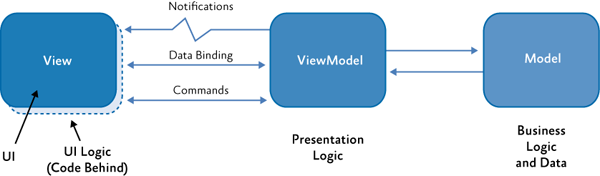
\includegraphics[width=1\linewidth]{mvvm.png}
  \caption{Illustration of the connection between view, model and
    viewmodel. From \cite{mvvm}}\label{fig:mvvm}
\end{figure}

The benefits of MVVM is that it provides a clean template for
separating the view logic from the business logic and from the data
layer.

This pattern is used mainly because the frameworks used on the client
and server are designed to be structured using this pattern. Other
similar patterns such as Model View Controller (MVC) could
theoretically also have been used, but doing so would go against some
of the principles the frameworks used are based upon.

\section{Singleton Pattern}

The singleton pattern is used whenever there should only ever be one
instance of a class \cite{skeet2013c}. The pattern is often implemented as a static
method on the class, that instantiates the class on the first call,
and on later calls returns the created instance of the class. In
\cref{fig:singleton}, the getSingleton would return the private field
singleton, making sure that the singleton field is initialized.

\begin{figure}
  \centering
  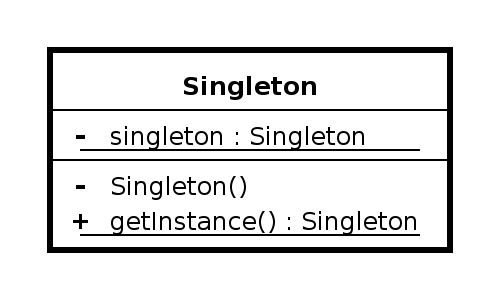
\includegraphics[width=0.7\linewidth]{singleton.png}
  \caption{Class diagram showing the important properties of a
    singleton class.}\label{fig:singleton}
\end{figure}

This pattern is used in SpotifyDotNet, the libspotify wrapper, used in
this project. Because it is only possible to be logged in one user at
a time, the SpotifyLoggedIn class implements the singleton pattern.

\section{Dependency Injection}

Dependency Injection is a design pattern that helps to reduce coupling
between different components in a software program \cite{injection}. The main idea is
to have components not depend on concrete dependencies but instead
depend on abstractions of dependencies. Doing this, dependencies can
be dynamically changed during runtime as long as their abstractions
match up.

In this project the StructureMap framework\footnote{http://docs.structuremap.net/} is used to reduce
boilerplate and ease the implementation of Dependency
Injection. StructureMap needs to be set up when the application
starts. That is, every dependency abstraction has to be mapped to a
concrete dependency. The dependency abstractions are modelled using
C\# interfaces. An example of an abstraction can be seen in
\cref{fig:dep_abstraction}. See \cref{fig:dependencyInjection}. The
builder class in this figure is the equivalent of the StructureMap
framework. It creates Client Class, while at the same time injecting a
concrete dependency, in this example the Service1, into Client Class' constructor. However Client
Class does not know it uses a concrete dependency. It is only aware of
the abstract dependency of IService1.

\begin{figure}
  \centering
  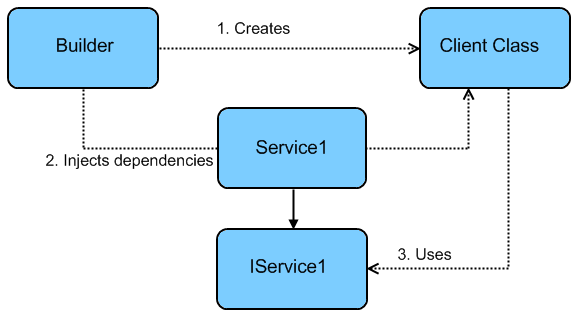
\includegraphics[width=1\linewidth]{DependencyInjection.png}
  \caption{An overview of dependency injection.}\label{fig:dependencyInjection}
\end{figure}

\begin{lstlisting}[caption = {Abstraction of a dependency abstraction
    using C\# interfaces. A concrete dependency has to implement the
    methods described in the abstraction.}, label={fig:dep_abstraction}]
public interface IPlaylistService
    {
        Track FindTrack(string trackUri);
        void Add(Track track);
        ConcurrentBagify<Track> Tracks { get; }
        int CalcTScore(Track track);
        Track NextTrack();
    }
\end{lstlisting}

To make use of a dependency in a component, the abstraction of the
dependency just has to be a parameter to the constructor of the
component. The StructureMap framework will then automatically inject
the concrete dependency that was mapped to the abstraction of the
dependency into the component. An example of this can be seen in
\cref{fig:injection}. So by using dependency injection, no component
has ever any knowledge of which concrete dependency it is using. The
component only knows that it depends on an abstraction of a
dependency. This property leads to several benefits, including
modularity of the code. That is, a whole dependency can be swapped for
another dependency as long as they both implement the abstract
dependency model.

\begin{lstlisting}[caption = {Dependency Injection through class
    constructors. IPlaylistService, IUserService and IPlaybackService
    are all abstractions of dependencies.}, label={fig:injection}]
public VoteService(IPlaylistService playlistService, IUserService userService, IPlaybackService playbackService) {
            _playbackService = playbackService;
            _playlistService = playlistService;
            _userService = userService;
        }
\end{lstlisting}
